\chapter{Theory}
\label{sec:theory}

\section{Kinetic theory}
% TODO: Skriv en litt generell intro.
% Boltzmannlikningen
% Antakelser
% Enskogteori
% Likevekt

\section{Hard-sphere fluids}
Hard-sphere (HS) fluids are fluids consisting of spherical particles 
interacting via the non-continuous potential 
\[
    \label{eq:hard_sphere_potential}
    u(r) = 
    \begin{cases}
        \infty, & r < \sigma \\
        0, & r > \sigma.
    \end{cases}
\]
$u$ is the interaction potential between two particles, 
$r$ is the distance between them, and $\sigma$ is 
the diameter of the particles. This potential makes 
it possible to analytically describe certain fluid 
properties using statistical mechanics. The HS 
potential is especially useful when modeling 
transport properties such as viscosity.


\section{Transport properties}
% TODO: Fyll inn tekst her.
% Nevn noe av Enskog-informasjonen fra neste seksjon her.
% Generelt om transportegenskaper, enskogteori som en metode for å finne dem
% Kanskje nevne andre metoder for å regne ut transportegenskaper?
% Viskositet som transportegenskap


\section{The viscosity of hard-sphere fluids}
One expression for the viscosity of HS fluids 
is the Enskog equation. This equation applies 
to one-component HS fluids consisting only of 
particles with the same mass $m$ and radius 
$\sigma$. The viscosity of such fluids is 
\cite{ref:pippo:composition_dependence}
\[
    \label{eq:enskog_viscosity}
    \eta(\rho,T) 
        = \eta_0 \left[g^{-1}(\sigma) 
        + 0.8\, V_{\text{excl}}\,\rho 
        + 0.776 \,V_{\text{excl}}^2 \,\rho^2 g(\sigma) 
        \right].
\]
%\[
%    \begin{split}
%        \eta(n,T)
%            &= \frac{\eta^0}{\chi} (1+\frac{1}{2} \alpha \chi n)^2 + \frac{3}{5} \bar{\omega}, \quad \text{where}\\
%        \alpha
%            &= \frac{8}{15} \pi \sigma^3, \quad \text{and} \\
%        \bar{\omega}
%            &= \frac{4}{9} n^2 \sigma^4 \chi \sqrt{\pi m \kB T}.
%    \end{split}
%\]
Here, 
\[
    \eta_0 = \eta(0, T) = 
    \frac{5}{16\sigma^2} \sqrt{\frac{m \kB T}{\pi}}
\]
is the viscosity of the fluid in the zero-density 
limit. $V_{\text{excl}}$, the excluded volume, 
is the part of the fluid which a particle cannot 
occupy, because it is occupied by other particles. 
$V_{\text{excl}}$ is commonly assumed to be the 
volume of all particles in the fluid. This however, 
is only correct in the zero-density limit. 
% When the fluid density is higher, 
The space in between particles may also be unavailable.
% TODO: Make a figure.

Lastly, in equation \eqref{eq:enskog_viscosity}, 
$g(\sigma)$ is a radial distribution function at 
contact.  $g(\sigma)$ is the probability distribution 
of particles around one particle in the fluid. 
This determines how the collision frequency depends 
on the density of the fluid. $g(\sigma)$ can be 
found for example using the system's equation of 
state, as done in \cite{ref:pippo:composition_dependence}.
This method is referred to as Modified Enskog Theory.

% Deler av dette kan også nevnes i seksjonen om transportegenskaper. 
% Det er et generelt problem det du beskriver om MFT (mean free time).

In Enskog theory, a central assumption is that 
there is no correlation between different collisions. 
This assumption is known as molecular chaos. 
This means that the mean free time between 
collisions is much larger than the collision 
duration. The assumption of molecular chaos 
breaks down at high fluid densities, when 
collisions are too frequent to be uncorrelated. 
Furthermore, it does not work for real fluids 
with long range continuous interaction potentials,
since long range interactions make the particles 
highly correlated. However, the assumption of 
molecular chaos is more acceptable for low 
density HS-fluids. 


\section{Viscosity of hard-sphere fluid mixtures}
The Enskog equation (equation \eqref{eq:enskog_viscosity}) 
was generalized by Thorne to describe two-component fluid 
mixtures\cite{ref:chapman:non_uniform_gases}.
A further generalization to mixtures of arbitrary 
component numbers has been performed by Tham and 
Gubbins\cite{ref:tham:fluid_mixtures}. The results 
are outlined below, as presented in 
\cite{ref:pippo:composition_dependence}.

The viscosity of a dense binary mixture 
of two hard-sphere fluids is given by
\[
    \label{eq:thorne_viscosity}
    \eta_{\text{mix}} 
        = \left(
            \frac{y_1^2}{H_{11}} 
            + \frac{y_2^2}{H_{22}} 
            - \frac{2 y_1 y_2 H_{12}}{H_{11} H_{22}}
        \right)
        \left(
            1 - \frac{H_{12}^2}{H_{11} H_{22}}
        \right)^{-1}
        + \frac{3}{5} \bar{\omega}_{\text{mix}},
\]
where
\[
    y_1 
        = x_1 \left(
            1   + \frac{1}{2} x_1 \alpha_{11} \chi_{11} n 
                + \frac{m_2}{m_1 + m_2} x_2 \alpha_{12} \chi_{12} n
        \right), 
\]
and
\[
    \begin{split}
        H_{12} &= H_{21}
                =   -\frac{2 x_1 x_2 \chi_{12}}{\eta^0_{12}}
                    \cdot \frac{m_1 m_2}{(m_1 + m_2)^2}
                    \left( \frac{5}{3A^*_{12}} - 1 \right), \\
        H_{11}
                &=  -\frac{x_1^2 \chi_{11}}{\eta^0_1}
                    +\frac{2 x_1 x_2 \chi_{12}}{\eta^0_{12}}
                    \cdot \frac{m_1 m_2}{(m_1 + m_2)^2}
                    \left( \frac{5}{3A^*_{12}} + \frac{m_2}{m_1} \right). \\
    \end{split}
\]
$y_2$ and $H_{22}$ follow from exchanging the subscripts in $y_1$ and $H_{11}$ 
respectively.
$A^*_{12}$ is a dimensionless ratio of collision integrals (of type ${ij}$).
For hard spheres, $A^*_{12}$ is exactly unity, and for other forms of 
interaction, it is close to unity. % Source here is de Pippo. Should I point that out?

$\chi_{ij} = \chi_{ji}$ are radial distrubution 
functions for molecules of type $i$ colliding 
with molecules of type $j$.
They correspond to the one-component radial 
distribution function $g(\sigma)$ in equation 
\eqref{eq:enskog_viscosity}.
Finally, $\bar{\omega}_{\text{mix}}$ can be written
\[
    \begin{split}
        \bar{\omega}_{\text{mix}} 
            &= x_1^2 \bar{\omega}_{11} 
            + x_1 x_2 \bar{\omega}_{12} 
            + x_2^2 \bar{\omega}_{22}, \text{where}\\
        \bar{\omega}_{ij} 
            &= \frac{4}{9} n^2 \sigma_{ij}^4 \chi_{ij} 
            \sqrt{\frac{2\pi m_1 m_2 \kB T}{m_1 + m_2}} 
            \text{for} i,j = 1,2.
    \end{split}
\]

% TODO: Elaborate on this, after discussing with Roberto.
%       In particular, say something about the physical meaning of every
%       "Russian doll" in the equation.

% TODO: Should I include the multi-component equation as well?
%       Or maybe just include one and many components, and skip two-component?
%       ANSWER: Start with multi-component, then reduce to two.
%       COMMENT TO ANSWER: Since the two-component version is more important
%       to this project, and since it was derived first, I think it's more
%       natural to present the two-component equation first, like Pippo does.

It is instructive to demonstrate how the two-component 
Thorne equation \eqref{eq:thorne_viscosity} reduces to 
the one-component Enskog equation \eqref{eq:enskog_viscosity}.
This is done by setting the density of either of the 
components to zero. Setting \(x_2 = 0\), so that 
\(y_2, \omega_\text{mix} = x_1^2\bar{omega}_{11}\)
gives 
\[
    H_{ij} = 
    \begin{bmatrix}
        H_{11}  & 0 \\
        0       & 0
    \end{bmatrix}.
\]
Now, equation \eqref{eq:thorne_viscosity} reduces to 
\[
    \eta_{\text{mix}} 
        = \frac{y_1^2}{H_{11}} 
        + \frac{3}{5} \bar{\omega}_{\text{mix}}
        = \frac{\eta^0_1}{\chi_{11}} \left(
            1   + \frac{1}{2} x_1 \alpha_{11} \chi_{11} n 
        \right)^2
        + x_1^2\bar{\omega}_{11}
\]
Renaming the factors, this equals
\[
    \begin{split}
    \eta_{\text{one}} 
        &= \frac{\eta^0}{g(\sigma)} \left[
            1+\frac{1}{2} \alpha g(\sigma) \rho
        \right]^2
        + x^2\bar{\omega} \\
        %&= \frac{\eta^0}{g(\sigma)}\left[
        %    1+\frac{1}{2} \alpha g(\sigma) \rho 
        %    + \frac{1}{4} \alpha^2 g^2(\sigma) \rho^2
        %\right] \\
        &= \eta^0\left[
            g^{-1}(\sigma) 
            + \frac{1}{2} \alpha \rho 
            + \frac{1}{4} \alpha^2 g(\sigma)
        \right]
        + x^2\bar{\omega}, \\
    \end{split}
\]
Lastly, 
\[
    \begin{split}
    \alpha
        &= \frac{8}{15} \pi \sigma^3, \quad \text{and} \\
    \bar{\omega}
        &= \frac{4}{9} \rho^2 \sigma^4 g(\sigma) \sqrt{\pi m \kB T}
    \end{split}
\]
is inserted, and it is assumed that                 % TODO: Calculate this by hand!
\(V_{\text{excl}} = \frac{N \pi \sigma^3}{6}\) 
is the total volume of the particles in the fluid.
This gives equation \eqref{eq:enskog_viscosity}
\[
    \eta 
        = \eta_0 \left[g^{-1}(\sigma) 
        + 0.8   \, V_{\text{excl}}      \,\rho 
        + 0.776 \, V_{\text{excl}}^2    \,\rho^2 g(\sigma) 
        \right].
\]

\section{Simulation of hard-sphere fluids}
Several methods exist for simulating fluids 
consisting of rigid spheres. They can be 
divided into two categories, namely Monte 
Carlo (MC) models, and molecular dynamics 
(MD) models. MC methods sample statistical 
ensembles using random walk,  % TODO: Find a better term than random walk.
while MD methods use Newton's equations of 
motion to compute the deterministic path 
of a large collection of particles.

Monte Carlo methods are typically easier to 
use with hard-sphere potentials, but can not 
be used to compute transport coefficients. 
% Can't, or can with difficulty? 
% That's an important distinction.
Molecular dynamics methods on the other 
hand, allow calculating dynamical and 
out-of-equilibrium properties of a system. 
To compute the viscosity of a system, 
MD methods should therefore be used. 

This section therefore gives an introduction 
to molecular dynamics, focusing especially on 
molecular dynamics for hard and pseudo-hard 
spheres \cite{ref:allen:MD_sim}.

% Mer generelt om MD (inkl hendelsesdrevent)
\section{Event-driven molecular dynamics simulation}
A simple method for performing molecular 
dynamics simulations with hard sphere in 
is an \emph{event-driven simulation}. 
Key elements of this simulation method 
is outlined below.

Compute the time until a collision occurs, for all particles in the system.
All collisions are stored in a list containing at least information about
the time of the collision, and the identity of the two involved particles.
Then, the time until the earliest collision is identified by searching through the list.
Using Newton's equations of motion, all atoms are propagated freely until
the collision happens.
Through conservation laws, the colliding particles' velocities are then updated.
Their next collisions are then added to the list of upcoming collisions.
This process is repeated, and all atom positions are updated with the time 
until the next collision in the list.

It should be noted that after a collision happens, other collisions involving
either of the two particles will be invalid.
These should be discarded from the list.

\section{Continuous potential MD simulation methods}
Several powerful and efficient molecular dynamics 
programmes are easily available, including LAMMPS, 
GROMACS, DL\_POLY and NAND. % TODO add references.  
These do, however, not handle discontinuous potentials.
Thus, the event-driven method is not supported by 
any of these programmes \cite{ref:allen:MD_sim}. In 
order to utilize the efficiency of the available MD 
software, it is more convenient to use a different 
method. The hard sphere potential can be approximated 
with a steep but continuous interaction potential 
instead. Then, the particle positions are updated 
using numerical integration methods with short, 
finite time steps.

Additionally, once there are long-range 
interaction forces between particles, then 
interactions occur at all times. In this 
case, the event driven simulation does not 
work, and integration methods are required. 
Therefore, continuous potential modelling 
is much more useful for realistic fluid models.

Several potentials are possible to use as 
hard-sphere approximations. The Lennard-Jones 
potential 
\[
    \label{eq:lennard_jones_potential}
    u_{\text{LJ}}(r) = 
        4 \epsilon \left[
            \left(\frac{\sigma}{r}\right)^{12} -
            \left(\frac{\sigma}{r}\right)^{6}
        \right]
\]
is a well-known example of historical importance.
Here, $\epsilon$ is the well depth -- the minimal value of 
the potential. As in \eqref{eq:hard_sphere_potential}, 
$\sigma$ and $r$ are the diameter and relative distance of 
the interacting particles.

If the attractive part, 
$\left[- \left(\frac{\sigma}{r}\right)^{6}\right]$
in equation \eqref{eq:lennard_jones_potential} 
is removed from the potential, then $u_{\text{LJ}}(r)$ 
can represent purely repulsive interactions. This is done 
by shifting the potential upwards by its minimal value 
$\epsilon$ and cutting it off there. Thus, the potential 
is exactly zero once it has reached its minimum. The 
resulting potential
\[
    \label{eq:WCA_potential}
    u_{WCA}(r) = 
    \begin{cases}
        4 \epsilon \left[
            \left(\frac{\sigma}{r}\right)^{12} -
            \left(\frac{\sigma}{r}\right)^{6}
        \right]
        + \epsilon,
            & r < 2^\frac{1}{6} \sigma\\
        0,  & r > 2^\frac{1}{6}\sigma.
    \end{cases}
\]
is known as a WCA-potential.
This serves as an approximation to a hard sphere potential.
% This is explained below. 
% TODO: Move the explanation here, so that everything is chronological.

Increased computer efficiency makes it more appropriate 
to use steeper potentials than the WCA-potential.
In particular, Jover et al. \cite{ref:jover:pseudo_hard} 
has proposed the Mie (or generalized Lennard-Jones) potential
\[
    u_{\text{Mie}}(r) = 
        \frac{\lambda_r}{\lambda_r - \lambda_a}
        \left(\frac{\lambda_r}{\lambda_a}\right)
        ^{\frac{\lambda_a}{\lambda_r - \lambda_a}}
        \epsilon \left[
            \left(\frac{\sigma}{r}\right)^{\lambda_r} -
            \left(\frac{\sigma}{r}\right)^{\lambda_a}
        \right],
\]
as an approximation to the hard-sphere interaction potential.
% What's a better word than "strength"??
The exponents $\lambda_r$ and $\lambda_a$ define the strength 
of the repulsive and attractive parts of the potential.

Cutting and shifting the $u_{\text{Mie}}$ potential as done in equations
\eqref{eq:lennard_jones_potential} and \eqref{eq:WCA_potential},
gives a steep non-negative potential of the form
\[
    u_{(\lambda_a, \lambda_b)}(r) = 
    \begin{cases}
        \frac{\lambda_r}{\lambda_r - \lambda_a}
        \left(\frac{\lambda_r}{\lambda_a}\right)
        ^{\frac{\lambda_a}{\lambda_r - \lambda_a}}
        \epsilon \left[
            \left(\frac{\sigma}{r}\right)^{\lambda_r} -
            \left(\frac{\sigma}{r}\right)^{\lambda_a}
        \right]
        + \epsilon,
            & r < \sigma \left(
                \frac{\lambda_r}{\lambda_a}
            \right)^\frac{1}{\lambda_r - \lambda_a} \\
        0,  & r > \sigma \left(
                \frac{\lambda_r}{\lambda_a}
            \right)^\frac{1}{\lambda_r - \lambda_a},
    \end{cases}
\]
closely resembling that of an infinitely steep hard 
wall potential (equation \eqref{eq:hard_sphere_potential}).
This potential is referred to as a pseudo hard-sphere (PHS) potential.

Jover et al. chose the exponents \((\lambda_r, \lambda_a) = (50, 49)\), 
as a compromise between faithfulness of the pseudo hard representation 
towards the perfectly hard wall, and computational speed.
Higher exponents will produce a steeper repulsion. 
This however, comes at a cost. 
The steeper the potential, the shorter time steps are 
needed to ensure that the computations are precise.
% TODO: Definer hva presist betyr.
Therefore, steeper repulsions are computationally 
more expensive to simulate.

Writing it out for clarity, the Mie (50, 49)-potential has the form
\[
    u_{(50, 49)}(r) = 
    \begin{cases}
        50
        \left(\frac{50}{49}\right)^{49}
        \epsilon \left[
            \left(\frac{\sigma}{r}\right)^{50} -
            \left(\frac{\sigma}{r}\right)^{49}
        \right]
        + \epsilon,
            & r < \frac{50}{49} \sigma\\
        0,  & r > \frac{50}{49} \sigma.
    \end{cases}
\]

\begin{figure}[htbp]
    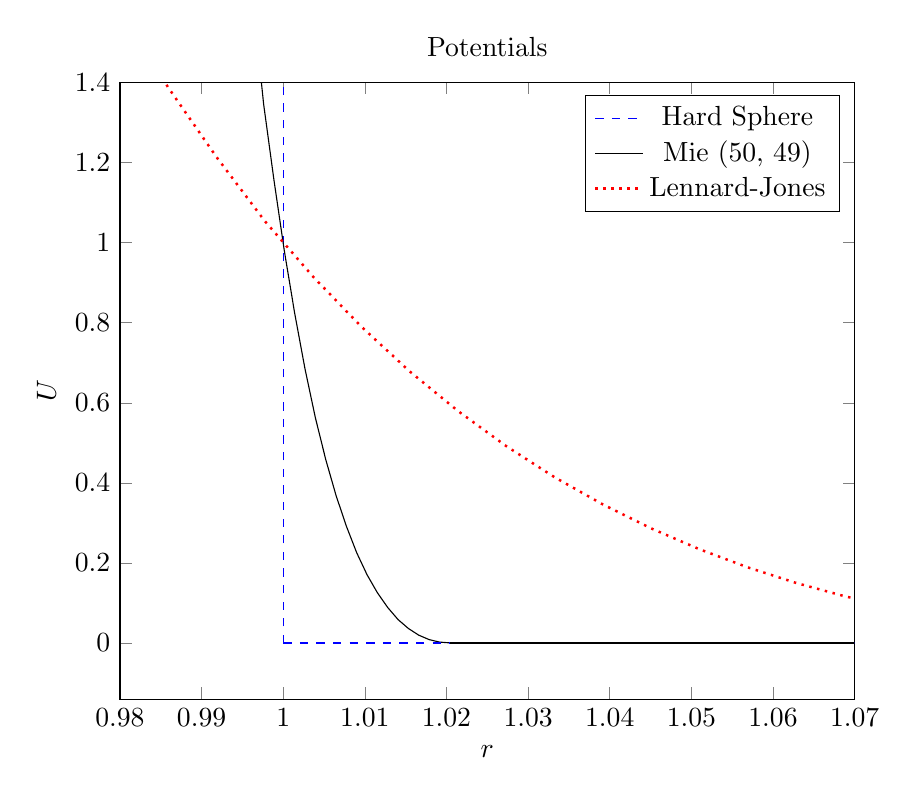
\begin{tikzpicture}
    \begin{axis}[
        title=Potentials,
        xlabel=$r$,
        ylabel=$U$,
        width=0.9\textwidth,
        ymax=1.4,
        xmin=0.98,
        xmax=1.07,
        cycle list = {
            color=blue,     style=dashed,   \\%
            color=black,    style=solid,    \\%
            color=red,      style=dotted,   line width=0.9pt,\\%
}
    ]
        % HARD SPHERE:
        \addplot+ [
            domain=0:1.1,
            mark=none,
            ] coordinates {(1,0) (1,2)};
            \addlegendentry{Hard Sphere}
        % MIE:
        \addplot+ [
            domain=0.99:1.0204,
            ]{50*(50/49)^49 * ((1/x)^50 - (1/x)^49) + 1.0};
            \addlegendentry{Mie (50, 49)}
        % LENNARD-JONES
        \addplot+ [
            domain=0.98:1.122,
        ]{4*((1/x)^12 - (1/x)^6) + 1};
        \addlegendentry{Lennard-Jones}
        % HARD SPHERE:
        \addplot+ [
            domain=1:1.1,
            mark=none,
        ] {0};
        % MIE:
        \addplot+ [
            color=black,
            domain=1.0204:1.1,
        ]{0};
        % LENNARD-JONES
        \addplot+ [
            domain=1.122:1.2,
        ]{0};
    \end{axis}
\end{tikzpicture}

    \caption{The cut-and-shifted WCA(50, 49)-potential 
            compared to the cut and shifted WCA(12, 6) 
            (Lennard-Jones) as well as the hard sphere 
            potential.
    }
\end{figure}

Pousaneh and de Wijn \cite{ref:pousaneh:shear_viscosity} 
have shown that such a pseudo-hard sphere potential 
can be used to model viscosity for a one-component hard-sphere fluid, 
and that the obtained viscosity is in agreement with Enskog theory.
% However, to the best of our knowledge, such a confirmation has not 
% been published for fluids of more than one component. 
% C: Dette er er ikke sjekket, men er jo delvis det du skal gjøre.


\section{Measuring the viscosity of a fluid in NEMD}
Müller-Plathe \cite{ref:mullerplathe:reversing_the_perturbation} 
has proposed a method of computing the viscosity of a fluid in 
nonequilibrium molecular dynamics (NEMD) simulations.
% TODO: Describe method, including figures.

Consider a rectangular box with sides of length \((L_x, L_y, L_z)\) 
with periodic boundary conditions.
The box contains a hard sphere fluid at equilibrium.
We divide the system into two equal slabs, their border 
being parallel to the $xy$-plane at height \(z = L_z/2\).
Now, we can define three parallel planes, at 
\(z = \{0, L_z/2, L_z\}\), which are the edges of the two slabs.
At these edges, we will control the velocity of the particles, 
making sure that the particles flow in the directions
\[
    \label{eq:velocity_directions}
    \hat{u}_x(z) =
    \begin{cases}
        +\hat{x}, \,z = L_z,    \\
        -\hat{x}, \,z = L_z/2,  \\
        +\hat{x}, \,z = 0,    \\
    \end{cases}
\]
as shown in figure (??). %TODO: Figure.
Here, \(u_x(z)\) denotes the average velocity component 
in $x$-direction, of the particles at height $z$.
The hat ``\(\,\, \hat{ } \,\,\)'' denotes 
directional vectors of length unity.

The particle flows are adjusted through an unphysical process known as a 
\textbf{reverse perturbation}\cite{ref:mullerplathe:reversing_the_perturbation},
as follows:

Find the particle in the \(z = 0\) slab edge with the lowest 
(most negative) velocity component in the \(+x\)-direction.
Correspondingly, find the particle in the \(z = L/2\) border 
with the largest velocity component in the \(+x\)-direction.
Then, swap the momenta of these two particles.
Repeat the process for the top slab, swapping the smallest momentum 
in the \(z = L\) edge with the largest momentum in the \(z = L/2\) edge.
This process is then repeated periodically.
The repeated reverse perturbations cause a velocity profile in the fluid,
as shown in figure (??). % TODO: Figure.
At the edges of the slabs, the velocity directions 
is given by equation \eqref{eq:velocity_directions}.

The velocity profile will cause a momentum flux in $z$-direction,
\[
    \label{eq:momentum_flux}
    j_z = -\eta \frac{\partial u_x}{\partial z}.
\]
This flux is proportional to the viscosity of the fluid, and is measurable.
Thus, the viscosity can be calculated from velocity data generated in the 
MD simulation.

\begin{figure}
    \begin{center}
        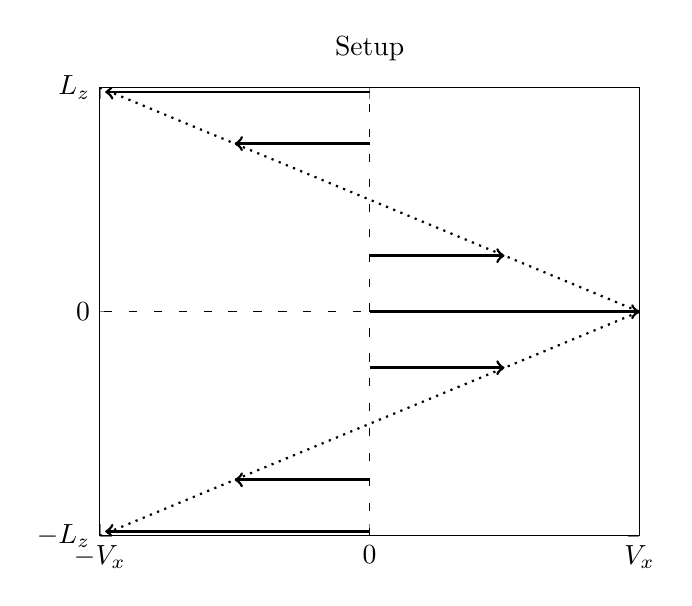
\begin{tikzpicture}
\def\V{1.0}
\def\Lz{1.0}
\begin{axis}[
    title=Setup,
    xmin=-\V,
    xmax=\V,
    ymin=-1.00*\Lz,
    ymax=1.00*\Lz,
    xtick={-\V,0,\V},
    ytick={-\Lz,0,\Lz},
    xticklabels={$-V_x$, $0$, $V_x$},
    yticklabels={$-L_z$, $0$, $L_z$},
]
    \addplot[ % Upper half velocity profile
        domain=-\V:\V,
        dotted,
        line width=0.8pt,
        ] {-\Lz/(2*\V)*x+\Lz/2};
    \addplot[ % Lower half velocity profile
        domain=-\V:\V,
        dotted,
        line width=0.8pt,
        ] {\Lz/(2*\V)*x-\Lz/2};
    \addplot[ % Middle plane of box
        domain=-2*\V:2*\V,
        loosely dashed,
        ] {0};
    \addplot[ % Middle plane of box
        loosely dashed,
        ] coordinates {(0,-2*\Lz) (0,2*\Lz)};
        \draw [-to, line width=1pt] (0, 0.25)   -- (0.5,    0.25);
        \draw [-to, line width=1pt] (0, -0.25)  -- (0.5,    -0.25);

        \draw [-to, line width=1pt] (0, 0.75)   -- (-0.5,   0.75);
        \draw [-to, line width=1pt] (0, -0.75)  -- (-0.5,   -0.75);

        \draw [-to, line width=1pt] (0, 0.98)      -- (-0.98,   0.98);
        \draw [-to, line width=1pt] (0, -0.98)     -- (-0.98,   -0.98);

        \draw [-to, line width=1pt] (0, 0)      -- (1.0,   0);
\end{axis}
\end{tikzpicture}

        \caption{The setup of the Müller-Plathe experiment.}
    \end{center}
\end{figure}
